% !TEX root = ../main.tex

\chapter{Background}
\label{chapter:Background}
In this thesis machine learning will be defined as the guided search for candidate functions $f^*: X \to Y$ to maximize the expectation of an objective function 
${g: X \times Y \to \mathbb{R}}$ using a signal function $g^*$, which is available during training time:
\begin{equation}
    \label{general_learning_paradigm}
    \begin{aligned}
        f^* &= \arg\max_{f} \mathbb{E}_{x \sim D}[g(x,f(x))] \\
        f^* &\approx f' = \arg\max_{f} \mathbb{E}_{x \sim D_{train}}[g^*(x,f(x))]
    \end{aligned}
\end{equation}

Commonly, $g^*$ is either a (negative) loss or a (positive) reward.

Following the book "Pattern Recognition and Machine Learning" \cite{bishop} there are three learning paradigms common in machine learning: 
\begin{itemize}
	\item Supervised Learning
	\item Unsupervised Learning
	\item Reinforcement Learning
\end{itemize} .

\section{Supervised Learning}
\label{section:super_learn}
Supervised learning is a learning paradigm where the input-output pairs $(x,y) \in X \times Y$ are given, and the goal is to learn a function 
$f^*$ that maps inputs $x \in X$ to outputs $y \in Y$. The objective function is typically a loss function that measures the difference between 
the predicted output $f(x)$ and the true output $y$.

Formally, the signal or loss function $L = g^*$ is defined on a training set $D_{train} = {(x_i,y_i)}_{i=1}^n$ where $x_i \in X$ and $y_i \in Y$. Using the 
labels, it computes a loss between the output of a function $f(x_i)$ and a desired output $y_i$. The signal function is shaped such that optimizing $f$ for $L$ 
over $D_{train}$ should be aligned with optimizing $f$ for $g$ over $D$:

\begin{equation}
\begin{aligned}
f^* &= \arg\min_{f} \mathbb{E}_{(x,y) \sim D}[g(f(x), y)] \\
f^* &\approx f' = \arg\min_{f} \mathbb{E}_{(x,y) \sim D_{train}}[L(f(x),y)] = \arg\min{f} \frac{1}{n}\sum_{i=1}^n L(f(x_i),y_i)
\end{aligned}
\end{equation}


Supervised learning can be used for a variety of tasks, including classification, regression, and sequence prediction. In classification, 
the goal is to predict a discrete class label $y \in {1,2,\ldots,K}$ for a given input $x$. In regression, the goal is to predict a continuous 
output $y \in \mathbb{R}$ for a given input $x$. In sequence prediction, the goal is to predict a sequence of outputs $y_1,\ldots,y_T$ for a 
given input sequence $x_1,\ldots,x_T$ \cite[chapter~4]{bishop} \cite[chapter~5, chapter~6]{Goodfellow}.

\section{Unsupervised Learning}
\label{section:unsup_learn}
Unsupervised learning is a learning paradigm where the input data is unlabeled and the goal is to discover underlying patterns or structure in the data.
The objective function in unsupervised learning is typically not based on a pre-defined notion of correctness, but rather on measures of statistical
independence or data compression.\\

Unsupervised learning can be used for a variety of tasks, including clustering, density estimation, dimensionality reduction, and anomaly detection.
It is also often used as a pre-processing step in supervised learning, where the goal is to learn a representation of the input data that is more informative
for the downstream task \cite[chapter~9]{bishop} \cite[chapter~5]{Goodfellow}. 

\section{Reinforcement Learning}
\label{section:rl}

Reinforcement learning is a learning paradigm where an agent interacts with an environment and learns to take actions that maximize a 
cumulative reward signal. In this paradigm, the input $x$ is typically the state $s$ of the environment, the output $y$ is the action $a$ taken by the agent, 
and the the objective function $g$ is a reward signal $r$.

The agent learns a policy $\pi: S \to A$ that maps states to actions, in order to maximize the expected cumulative reward:

\begin{equation}
    \label{rl_objective}
    \begin{aligned}
    \pi^* &= \arg\max_{\pi} \mathbb{E}_{\tau \sim p(\tau | \pi)} \left[ \sum_{t=0}^T \gamma^t r_t \right] \\
    \approx \pi' = \arg\max_{\pi} \frac{1}{N} \sum_{i=1}^N \left[ \sum_{t=0}^{T_i} \gamma^t r_{i,t} \right]
    \end{aligned}
\end{equation}

where $\tau = (s_0, a_0, r_0, s_1, a_1, r_1, \ldots, s_T, a_T, r_T)$ is a trajectory, $p(\tau | \pi)$ is the probability of a trajectory 
under policy $\pi$, $\gamma \in [0,1]$ is a discount factor that controls the importance of future rewards, and $N$ is the number of trajectories sampled.

\subsection{Classification of Reinforcement Learning}
\begin{minipage}{\textwidth}
\begin{itemize}

    \item \textbf{Model type:}
    \begin{itemize}
    \item Model-based: the algorithm explicitly models the dynamics of the environment.
    \item Model-free: the algorithm learns a policy without explicitly modeling the environment.
    \end{itemize}
    \item \textbf{Action/Observation space:}
    \begin{itemize}
    \item Continuous: the action/observation space is continuous, typically represented by a real-valued vector.
    \item Discrete: the action/observation space is discrete, typically represented by a finite set of actions.
    \end{itemize}
    \item \textbf{Policy type:}
    \begin{itemize}
    \item On-policy: the algorithm learns the optimal policy while using the same policy to collect experience.
    \item Off-policy: the algorithm learns the optimal policy while using a different policy to collect experience.
    \end{itemize}
    \item \textbf{Reward type:}
    \begin{itemize}
    \item Dense reward: the agent receives a reward signal for every time step in the environment.
    \item Sparse reward: the agent receives a reward signal only for certain time steps in the environment.
    \end{itemize}
    \item \textbf{Time horizon:}
    \begin{itemize}
    \item Infinite horizon: the algorithm aims to maximize the expected sum of rewards over an infinite time horizon.
    \item Finite horizon: the algorithm aims to maximize the expected sum of rewards over a fixed time horizon.
    \end{itemize}
    \item \textbf{inference type:}
    \begin{itemize}
    \item Probabalistic inference: the algorithm samples actions according to a probability distribution.
    \item Deterministic inference: the algorithm chooses an action deterministicly.
    \end{itemize}
    \end{itemize}
\end{minipage}

\section{Markov Decision Processes}
Markov Decision Processes (MDPs) are a mathematical framework used to model decision-making processes that occur in a sequence. They provide a useful 
context to develop reinforcement learning algorithms.

An MDP is defined as a tuple $(S, A, T, R, \gamma)$, where:
\begin{itemize}
    \item $S$ is the set of possible states in the system
    \item $A$ is the set of possible actions that can be taken in each state
    \item $T$ is the transition function that specifies the probability of moving from one state to another given a certain action
    \item $R$ is the reward function that specifies the immediate reward obtained after taking a certain action in a certain state
    \item $\gamma$ is the discount factor that determines the importance of future rewards relative to immediate rewards
\end{itemize}

The transition function $T$ is defined as:

$$T(s, a, s') = \mathbb{P}(s_{t+1}=s' \mid s_t=s, a_t=a)$$

This function specifies the probability of moving from state $s$ to state $s'$ after taking action $a$. The reward function $R$ is defined as:

$$R(s, a) = \mathbb{E}[r_{t+1} \mid s_t=s, a_t=a]$$

This function specifies the expected immediate reward obtained after taking action $a$ in state $s$. The discount factor $\gamma$ is a 
parameter that determines the importance of future rewards relative to immediate rewards. It is typically a value between 0 and 1, where 0 means that 
only immediate rewards are important and 1 means that future rewards are equally important. \\

Importantly, the transition function $T$ satisfies the markov property. The Markov property characterizes stochastic processes where the future state of the 
process depends only on the current state and not on any past states. Formally, a stochastic process has the Markov property if, 
for all time steps $t$, states $s_t$, and actions $a_t$, the following condition holds:

\begin{equation}
    P(s_{t+1} \mid s_t, a_t, s_{t-1}, a_{t-1}, \ldots, s_1, a_1) = P(s_{t+1} \mid s_t, a_t)
\end{equation}

\begin{figure}
    \centering
    \begin{tikzpicture}[node distance=2cm]
        font=\fontsize{20};
        % Define nodes
        \node (s1) [circle, draw, fill = green!30] {$s_1$};
        \node (t1_2) [rectangle, draw, right of=s1, xshift=1.5cm] {$T(s_2|s_1, a_1)$};
        \node (s2) [circle, draw, fill = green!30, right of = t1_2, xshift=1.5cm] {$s_2$};
        \node (t2_3) [rectangle, draw, right of=s2, xshift=1.5cm] {$T(s_3|s_2, a_2)$};
        \node (s3) [circle, draw, fill = green!30, right of = t2_3, xshift=1.5cm] {$s_3$};
        \node (r_1) [rectangle, draw, fill = {rgb,255:red,70;green,90;blue,70}, below of=t1_2] {$R(s_1, a_1)$};
        \node (r_2) [rectangle, draw, fill = {rgb,255:red,70;green,90;blue,70}, below of=t2_3] {$R(s_2, a_2)$};

        \node (policy_1) [diamond, draw, fill = yellow!30, above of = s1, yshift=1.5cm] {$\pi$};
        \node (policy_2) [diamond, draw, fill = yellow!30, above of = s2, yshift=1.5cm] {$\pi$};
        \node (policy_3) [diamond, draw, fill = yellow!30, above of = s3, yshift=1.5cm] {$\pi$};

        \draw [->, black!50, line width=2pt] (s1) -- node[midway, above] {} (policy_1);
        \draw [->, black!50, line width=2pt] (s2) -- node[midway, above] {} (policy_2);
        \draw [->, black!50, line width=2pt] (s3) -- node[midway, above] {} (policy_3);

        \draw [->, black!50, line width=2pt] (s1) -- node[midway, above] {} (t1_2);
        \draw [->, black!50, line width=2pt] (s2) -- node[midway, above] {} (t2_3);


        \draw [->, black!50, line width=2pt] (policy_1) -- node[black!100, midway, below] {$a_1$} (t1_2);
        \draw [->, black!50, line width=2pt] (policy_2) -- node[black!100, midway, below] {$a_2$} (t2_3);

        \draw [->, black!50, line width=2pt] (t1_2) -- node[midway, left] {} (s2);
        \draw [->, black!50, line width=2pt] (t2_3) -- node[midway, left] {} (s3);

        \draw [->, color={rgb,255:red,70;green,90;blue,70}, line width=2pt] (t1_2) -- node[midway, left] {} (r_1);
        \draw [->, color={rgb,255:red,70;green,90;blue,70}, line width=2pt] (t2_3) -- node[midway, left] {} (r_2);
    \end{tikzpicture}
  \caption{A MDP diagram with an agent that takes in states $s_t$ and outputs action $a_t$.}
\end{figure}
\section{Policy Gradient}
There are numerous ways to arrive at a policy that maximizes the reinforcment learning objective \ref{rl_objective}. For large or continuous action and observation spaces, a common approach is 
to parametrize the policy using a differentiable function. In this thesis we will be using neural networks for this task, as they have shown most promising results. The expectation over the cumulative 
reward $J = E[\sum_{t} \gamma^t r_t]$ with respect to a policy $\pi$ with parameters $\theta$ can be written as:

\begin{equation}
J(\theta) = \mathbb{E}_{\tau \sim p(\tau | \pi)} \left[ \sum_{t=0}^T \gamma^t r_t \right]
\end{equation}
where $\tau$ is a trajectory of state-action pairs, $p(\tau | \pi)$ is the probability of generating trajectory $\tau$ under policy $\pi$, and $\theta$ are the parameters of the policy $\pi$. 
$T$ can either be finite or infinite. If $T$ is infinite, $\gamma$ must be smaller then 1.

Our goal is to maximize $J(\theta)$ with respect to $\theta$. We can use the policy gradient theorem to compute the gradient of $J(\theta)$:
\begin{equation}
    \label{nabla_reinforce}
    \begin{aligned}
        \nabla_{\theta} J(\theta) = \mathbb{E}_{\tau \sim p(\tau | \pi)} \left[ \sum_{t=0}^T \nabla_{\theta} \log \pi(a_t|s_t;\theta) \cdot \sum_{t'=t}^T \gamma^{t'-t} r_{t'} \right]\\
        = \mathbb{E}_{\tau \sim p(\tau | \pi)} \left[ \sum_{t=0}^T \nabla_{\theta} \log \pi(a_t|s_t;\theta) \cdot  G_t\right]
    \end{aligned}
\end{equation}
With $G_t = \sum_{t'=t}^T \gamma^t' r_{t'}$ and $\pi(a_t|s_t;\theta)$ is the probability of taking action $a_t$ in state $s_t$ under policy $\pi$ with parameters $\theta$. 
$G_t$ represents the total discounted reward obtained after taking action $a_t$ in state $s_t$.

In practice we don't have access to the real expectation. Instead we sample n Trajectories and approximate the expectation.
A common choice is to sample one trajectory per update step. 
This finally gives us the gradient of the approximated expected reward with respect to the policy parameters $\theta$. We can use this gradient to update the parameters of the policy in the direction of steepest ascent. Specifically, we can use stochastic gradient ascent to update the policy parameters after observing a trajectory $\tau$:
\begin{equation}
    \label{reinf_update}
    \theta \leftarrow \theta + \alpha \nabla_{\theta} \log \pi(a_t|s_t;\theta) \cdot G_t
\end{equation}
where $\alpha$ is the learning rate. This update rule is used in the REINFORCE algorithm:

\begin{algorithm}[H]
    \SetAlgoLined
        \KwIn{Policy function $\pi_{\theta}(a|s)$, learning rate $\alpha$}
        \KwOut{Learned policy parameters $\theta$}
        Initialize policy parameters $\theta$;
        \While{not converged}{
            Sample a trajectory $\tau = (s_1, a_1, r_2, \dots, s_{T-1}, a_{T-1}, r_T, s_T)$ by following the policy $\pi_{\theta}$:\\
            \For{$t\leftarrow 1$ \KwTo $T$}{
                Compute the return starting from time $t$: \\
                $G_t = \sum_{k=t}^T \gamma^{k-t} r_k$ ;\\
                Compute the gradient of the log probability of taking action $a_t$ in state $s_t$: \\
                $\delta_{\pi(\theta)} = \nabla_{\theta}\log \pi_{\theta}(a_t|s_t)$; \\
                Compute the gradient estimate for this time step: \\
                $g_t \leftarrow G_t \delta_{\pi(\theta)}$;
                Update policy parameters using the gradient estimate:
                $\theta \leftarrow \theta + \alpha g_t$;
            }
        }
    \caption{REINFORCE algorithm with one trajectory per update}
\end{algorithm}
    
The algorithm collects 1 trajectory, computes the gradient estimate, and updates the policy parameters using stochastic gradient ascent. The algorithm continues to collect more trajectories and update the policy until convergence.


\section{Value Functions}

Value functions are a fundamental concept in reinforcement learning and are used to estimate the expected return of being in a particular state or taking a particular action. In this section, we will discuss the two main types of value functions in Markov decision processes (MDPs): state-value functions and action-value functions.
To clean up the notation, we will use upper case letters for functions, if the argument 
is implicit and lower case, if the argument is explicit.

\subsection{State-Value Function}

The state-value function $v_{\pi}(s)$ is the expected return when starting in state $s$ and following policy $\pi$ thereafter. It is defined as:

\begin{equation}
    v_{\pi}(s) = \mathbb{E}_{\tau \propto \pi}\left[\sum_{t=0}^{\infty} \gamma^t r_t \mid s_0 = s\right].
\end{equation}

$\mathbb{E}_{\tau \propto \pi}$ denotes the expected value under policy $\pi$.

The state-value function satisfies the Bellman equation, which expresses the relationship between the value of a state and the values of its successor states:

\begin{equation}
    \label{bootstrap_v}
    \begin{aligned}
        v_{\pi}(s) = \mathbb{E}_{\tau \propto \pi}\left[\sum_{t=0}^{\infty} \gamma^t r_t \mid s_0 = s\right] \\
        = \sum_{a \in \mathcal{A}} \pi(a \mid s) \left[ r(a,s)  \\
        + \gamma \sum_{s' \in \mathcal{S}} p(s' \mid s,a) \sum_{a' \in \mathcal{A}} \pi(a' \mid s') \left[ r(a',s') + \gamma ...\right] \right]\\
        = \sum_{a \in \mathcal{A}} \pi(a \mid s) \left[ r(a,s) +  \gamma \sum_{s' \in \mathcal{S}} p(s' \mid s,a) v_{\pi}(s')\right]
    \end{aligned}
\end{equation}

where $\mathcal{A}$ is the set of possible actions, $\mathcal{S}$ is the set of possible states, $p(s' \mid s,a)$ is the transition probability 
from state $s$ to state $s'$ under action $a$, $r(s,a,s')$ is the reward received when transitioning from state $s$ to state $s'$ under 
action $a$, and $\gamma \in [0,1]$ is the discount factor. This derivation assumes a discrete action space,
however it can be adapted for the continuous case by exchanging the summation with an integral over the probability density function.

\subsection{Action-State Value Function}

The action-state value function, also known as the Q-function, is the expected return when starting in state $s$, taking action $a$, and following 
policy $\pi$ thereafter. It is defined as:

\begin{equation}
    q_{\pi}(s, a) = \mathbb{E}_{\tau \propto \pi}\left[\sum_{t=0}^T \gamma^t r_t \mid s_0 = s, a_0=a\right]
\end{equation}

where $A_t$ is the action taken at time step $t$.

The action-state value function also satisfies the Bellman equation:

\begin{equation}
    \label{bmeq_q}
    q_{\pi}(s,a) = r(s,a) + \sum_{s' \in \mathcal{S}} p(s' \mid s,a) \left(\gamma \sum_{a' \in \mathcal{A}} \pi(a' \mid s') q_{\pi}(s',a')\right).
\end{equation}

Both value functions can be expressed in terms of the respective other value function using the Bellman equation:
\begin{equation}
    \label{q_from_v}
    q_{\pi}(s,a) = r(s,a) + \gamma \mathbb{E}_{s'\propto T(s,a,s')}\left[ v_{\pi}(s') \right]
\end{equation}

and 

\begin{equation}
    v_{\pi}(s) = \mathbb{E}_{a \propto \pi(\cdot|s)} \left[ q_\pi(s,a) \right]
\end{equation}



\section{Actor-Critic Algorithm}
\label{AC-Alg}
One problem with REINFORCE is, that $G_t$ is computed from the rollout of a whole trajectory. As the policy changes with respect to the update step, this update 
rule is off policy with high variance. An idea is to approximate the expectation over $G_t$ using another neural network, so that an update can be made after every step, 
rather then after the whole trajectory. This approximation is referred to as a "critic" in the actor critic method.
\subsection{Critic}
In this section, we will derive an expression to aproximate $G_t$ by using an iterative update step with guaranteed convergence.
Revisiting \ref{nabla_reinforce}: 
\begin{equation}
    \begin{aligned}
        \mathbb{E}_{\tau \sim p(\tau | \pi)} \left[ \sum_{t=0}^T \nabla_{\theta} \log \pi(a_t|s_t;\theta) \cdot  G_t\right]\\
        = \mathbb{E}_{s_0, a_0, ... ,s_T, a_T \propto \pi} \left[
            \sum_{t=0}^{T}\nabla_{\theta} log \pi_{\theta}(a_t|s_t) \mathbb{E}_{r_t...r_T \propto \pi} \left[ G_t \right]
        \right]
    \end{aligned}
\end{equation}
, where 
\begin{equation}
    \begin{align}
        \mathbb{E}_{s_t, a_t, r_t...s_T, a_T, r_T \propto \pi} \left[ G_t \right] \\
        = r(s_t,a_t) + \gamma \mathbb{E}_{s_{t+1} \propto T(s_{t+1}|s_t, a_t)}\left[\mathbb{E}_{a_{t+1} \propto \pi(\cdot|s_t)}  \left[q_{\pi}(s_{t+1},a_{t+1})\right]  \right]
        = q_{\pi}(s_{t},a_{t}).
    \end{align}
\end{equation}
This follows the derivation as in \ref{bootstrap_v} for the $Q$-value in the continuous case.

Plugging in the defintion of the $Q$-value recursively gives us the Bellman equation for $Q$-values:
\begin{equation}
q_{\pi}(s_t, a_t) = \mathbb{E}_{\tau \propto p(\tau|\pi)} \left[ r(s_t,a_t) + \gamma q_{\pi}(s_{t+1}, a_{t+1})\right]
\end{equation}
for the sequence $\tau = (s_0,a_0, s_1, a_1...) \propto \pi$.\\
We want to find a policy $\pi^*$ for which the $Q$-function is maximal.
\begin{equation}
    Q^* = \max_{\pi} \left[\mathbb{E}_{\tau \propto \p(\tau|\pi)} \left[ r + \gamma Q_{\pi} \right]\right]
\end{equation}

Updateing the $Q$-Value greedily by applying the operator $\mathcal{T}_Q^*$ is guaranteed to converge to the optimal $Q$-Value (see section \ref{opt_contr}):
\begin{equation}
    \begin{aligned}
        q_{i+1}(s_t, a_t) = (\mathcal{T}_Q^* q_i)(s_t, a_t) \\
        =\mathbb{E}_{s_{t+1} \propto p(s_{t+1}|s_t, a_t)} \left[r(s_t, a_t) + \gamma  \max_{a'} \left[  q_i(s_{t+1}, a_{t + 1}) \right]\right].
    \end{aligned}
\end{equation}

We don't have access to the true expected value, but we can approximate it by using rollouts of our current policy, similar to the REINFORCE algorithm. As this introduces noice, 
in temporal difference learning (TD-learning) we define a learning rate $\alpha$ to smooth the update of the $Q$-Value:
\begin{equation}
    q_{i+1}(s_t, a_t) = q_i(s_t, a_t) + \alpha\left[r(s_t, a_t) + \gamma \left( \max_{a'} q(s_{t+1}, a')\right) - q_i(s_t, a_t) \right]
\end{equation}
It is prooven that for a sufficiently small $\alpha$ this update rule will converge to the optimal $Q$-value \cite{Watkins1992}. From this expression we can define a parametric update step by minimizing 
the RSME $J_Q(\theta_{i})$ between $Q(\theta_{i-1})' = \mathcal{T}_Q^* Q(\theta_{i-1})$ and $Q(\theta_i)$:
\begin{equation}
    \begin{aligned}
        J_Q(\theta_{i}) = \mathbb{E}\left[\left( Q(\theta_{i-1})' - (\theta_i) \right)^2\right]\\
        = \alpha \mathbb{E}_{s_t, a_t}\left[\left( r(s_t, a_t) + \gamma \left( \max_{a'} q_{\theta_{i-1}}(s_{t+1}, a')\right) - q_{\theta_{i}}(s_t, a)\right)^2\right]
    \end{aligned}
\end{equation}

We can now use this error to update the parameters of the $Q_{\theta}$-function:
\begin{equation}
    Q(\theta_{i+1}) : \theta_{i+1} = \theta_{i} - \alpha \nabla J_Q(\theta_{i})
\end{equation}

\subsubsection{Optimality}
\label{opt_contr}

We will cover the proof of the existens and uniqueness of $V^*$. Then we will show it's optimality. The respective proofs for $Q^*$ are analogous and can be found for example in \cite{Watkins1992}.
Parts of this derivation follows \cite{optimality}.\\ \\

\textbf{Definition:}\\
Let $(X, d)$ be a complete metric space. A a map $\mathcal{T}:X \rightarrow X$ is called a contractor if there exists a factor $\gamma \in [0, 1)$ s.t.
\begin{equation}
    d(\mathcal{T}(x), \mathcal{T}(y)) \leq \gamma \cdot d(x,y) | x,y \in X.
\end{equation}
\\ \\

\textbf{Banach Fixed Point Theorem:}\\
Let (X,d) be a complete metric space and $\mathcal{T}:X \leftarrow X$ a contractor. 
Then $\mathcal{T}$ has a unique fixed point $x^* \in X$, s.t. $\mathcal{T}(x^*) = x^*$. The sequence $lim_{n \leftarrow \infty}\mathcal{T}^n(x)$ converges to $x^*$.\\ \\

\textbf{Value Iteration}\\
Let $X : v(s) \in \mathcal{R}$ and $d = ||X||_{\infty} = \max|X|$. \\
The value iteration operator $\mathcal{B}$ is defined as:
\begin{equation}
    (\mathcal{T}_{V}v)(s) = \max_{a \in \mathcal{A}} \left[  r(s,a) +  \gamma \sum_{s' \in \mathcal{S}} p(s' \mid s,a) \left( v(s')\right) \right]
\end{equation}
\textbf{Assertion}\\

$\mathcal{T}_{V}$ is a contrator under the $\infty$-norm.\\ \\

\textbf{Proof:}\\
Let $V_1$, $V_2$ be two value functions $V : S \times A \to \mathcal{R}$, $0 \leq \gamma < 1$ and $\mathcal{T}_{V}$ the value iteration operator, then:
\begin{equation}
    \label{contractor}
||\mathcal{T}_{V}V_1(s) - \mathcal{T}_{V}V_2(s)||_{\infty, s} = 
\end{equation}
\begin{equation}
    \left|\left| \max_a \left[ r(s,a) + \gamma \sum_{s'} p(s' \mid s,a) v_1(s')\right] - \max_{a'}\left[ r(s,a') + \gamma \sum_{s'} p(s' \mid s,a') v_2(s') \right] \right|\right|_{\infty, s}
\end{equation}
\begin{equation}
    \leq \left|\left|\max_a \left[ r(s,a) + \gamma \sum_{s'} p(s' \mid s,a) v_1(s') - r(s,a) - \gamma \sum_{s'} p(s' \mid s,a) v_2(s')\right]\right|\right|_{\infty, s}
\end{equation}
\begin{equation}
= \gamma \left|\left|\max_a \left[ \sum_{s'} p(s' \mid s,a) (v_1(s') -v_2(s'))\right]\right|\right|_{\infty, s}
\end{equation}
\begin{equation}
\leq \gamma \left|\left|\max_a \left[ \sum_{s'} p(s' \mid s,a) \cdot \max_{s''} (v_1(s'') -v_2(s''))\right]\right|\right|_{\infty, s}
\end{equation}

\begin{equation}
= \gamma \left|\left|\max_{s''} \left[ (v_1(s'') - v_2(s''))\right]\right|\right|_{\infty, s}
\end{equation}

\begin{equation}
= \gamma \left|\left|(v_1(s'') - v_2(s''))\right|\right|_{\infty, s''}
\end{equation}

\begin{equation}
= \gamma \left|\left|(v_1(s) - v_2(s))\right|\right|_{\infty, s}.
\end{equation}

This leaves us to show, that the fix point $V_n$ under the value iteration operator is also the maximum of the value function $V$.\\
$\mathcal{T}_{V}$ is a monoton increasing operator on $V$: 
\begin{equation}
    \begin{align}
        \mathcal{T}_{V}v(s) = \max_{a \in \mathcal{A}} \left[ r(s,a) + \gamma  \sum_{s' \in \mathcal{S}} p(s' \mid s,a) v(s')\right]\\
        \geq r(s,a') + \gamma  \sum_{s' \in \mathcal{S}} p(s' \mid s,a') v(s') |a' \in A.
    \end{align}
\end{equation}
As $V_n$ is monoton increasing and converges to a unique value, it will approach it's supremum. 
For any practical application, this means it converges to it's maximum.

\subsection{Actor}
In the derivation of the Bellman operator update rule $\mathcal{T}_{V}$ we used the $\max$-operator to choose the best action to ensure a monoton increasing 
value estimate. In practice this is again unfeasable for large or continuous action spaces. Instead, we want a parametrized $\pi$ that computes an action. 
Note that we only need a monoton increasing value estimate to guarantee asymptotic convergence. It can be shown that with sufficiently small scheduled update 
steps $\alpha(i)$, monoton stochasitc improvement is guaranteed for the update step:
\begin{equation}
    \pi_{\phi_{i+1}}: \phi_{i+1} \leftarrow \phi_i + \alpha(i) \left(
        \mathbb{E}_{s_0, a_0, ... ,s_T, a_T \propto \pi} \left[
            \sum_{t=0}^{T} \nabla_t \pi_{\phi_i} \right]
    \right)
\end{equation}
\begin{equation*}
    \text{with} \quad \nabla_t \pi_{\phi_i} = \nabla_{\theta} log \left( \pi_{\phi_i}(a_t|s_t)\right) \mathbb{E}_{a_t, s_t...a_T, s_T \propto \pi} \left[ Q_{\pi_{\phi_i}} \right] 
\end{equation*}
, where $Q_{\pi_{\phi}}$ is the fix point of the Bellman operator $\mathcal{T}_{Q_{\pi_{\phi}}}$:

\begin{equation}
    Q_{\pi_{\phi}} = \lim_{n \to \infty} Q^n_{\pi_{\phi}}
\end{equation}

\begin{equation*}
    \text{with}\quad q^{n+1}(s,a) = \mathcal{T}_{Q_{\pi_{\phi}}}q^n(s,a) = r(s,a) + \gamma \mathbb{E}_{\tau \propto {\pi_{\phi}}}[q^n(s_{t+1}, a_{t+1})]
\end{equation*}
with corresponding temporal difference term:
\begin{equation}
    \begin{aligned}
        J_{Q_{\pi_{\phi_i}}}(\theta_{i}) = \mathbb{E}\left[\left({Q_{\pi_{\phi_i}}}(\theta_{i-1})' - Q_{\pi_{\phi_i}}(\theta_{i}) \right)^2\right]\\
        = \alpha \mathbb{E}_{s_t, a_t}\left[\left( r(s_t, a_t) + \gamma \mathbb[E]_{a' \propto \pi_{\phi_i}}\left( q_{\theta_{i-1}}(s_{t+1}, a')\right) - q_{\theta_{i}}(s_t, a)\right)^2\right].
    \end{aligned}
\end{equation}
This defines two update steps, one for the policy and one for the critic. Commonly this approach is called deep deterministic policy gradient or DDPG \cite{https://arxiv.org/pdf/1509.02971.pdf}. Some algorithms don't use the $Q$ value for the update step of the policy, but a closely 
related value, called the advantage $A_t$ defined as $A_t = -V(s_t) + r_t + \gamma r_{t+1} + \cdots + \gamma^{T-t+1} r_{T-1} + \gamma^{T-t} V(s_T)$ \cite{A2C}. For the one step 
unroll of the rewards, this value becomes $A_t = Q(a_t, s_t) - V(s_t)$. 
Intuitively, the advantage $A$ is a measure for how good a specific action $a$ is compared to the average action taken by the current policy. 
A proof for the convergence and optimality of this estimator can be found in \cite{proof_A}.

\subsection{Soft Actor-Critic}
\label{SAC}
In the paper "Soft Actor-Critic" from Tuomas Haarnoja, et al. \cite{haarnoja2018soft} a new approach for exploration is introduces. Exploration vs. exploitation 
is a fundamental trade-off in reinforcement learning. On the one hand, an agent must exploit the current knowledge to maximize the cumulative reward it receives 
over the course of its interactions with the environment. On the other hand, the agent must explore new actions and states to improve its knowledge and avoid getting stuck in suboptimal policies. 
The balance between exploration and exploitation is crucial for the success of RL algorithms, and different methods aim to find a good compromise between them.

The soft actor-critic (SAC) algorithm extends the AC method by introducing a new objective that encourages the policy to be more stochastic. Specifically, the SAC algorithm maximizes a modified 
version of the expected cumulative reward that takes into account both the expected reward and the entropy of the policy. The modified objective is given by:

\begin{equation}
J(\pi) = \mathbb{E}_{s_t \sim \mathcal{D}, a_t \sim \pi}[r(s_t, a_t) + \alpha \mathcal{H}(\pi(\cdot|s_t))]
\end{equation}

where $\mathcal{D}$ is the replay buffer, $r(s_t, a_t)$ is the immediate reward for taking action $a_t$ in state $s_t$, and $\mathcal{H}(\pi(\cdot|s_t))$ is the entropy of the policy. The entropy 
encourages the policy to be more stochastic and explore different actions, while the temperature parameter $\alpha$ controls the trade-off between exploration and exploitation.

in the original mplementation, SAC uses two $Q$ value estimates and a $V$ value estimate. The V value is learned by 

\begin{equation}
    V_{\psi}(s_t) = \mathbb{E}_{a_t \sim \pi_{\phi(a_t|s_t)}}[q_\text{min}(s_t, a_t) - \alpha \log \pi_{\phi(a_t|s_t)}]
\end{equation}
, with the minimum value of the two $Q$ critics $Q_\text{min}$ to decrease the overestimation bias of critics in actor critic algorithms. 
Using this, the $Q$ values are trained with typical TD:

\begin{equation}
    \mathcal{J}(Q_{\theta_i}) = \mathbb{E}_{(s_t, a_t, r_t, s{t+1}) \sim \mathcal{D}}[(q_{\theta_i}(s_t,a_t) - y_t)^2]
\end{equation}

where $y_t = r(s_t, a_t) + \gamma \mathbb{E}_{s_{t+1} \sim p}[V(s_{t+1})]$ is the target value. 

The policy is updated to minimize the Kullback-Leibler (KL) divergence to the normalized $Q$-Values:
\begin{equation}
    \label{sac_pol_obj}
    J_\pi(\phi_{i}) = D_{KL} \left( \pi_{\phi_{i}}(\cdot|s_t) || \frac{\exp(Q_{min, {\theta_i}}(\cdot|s_t))}{\underset{a}{\sum}  \exp(Q_{\theta_i}(a|s_t))} \right).
\end{equation}

The KL divergence is a measure of the alikeness of two distributions $P(x)$ and $Q(x)$ over the same sample space $X$:
\begin{equation}
    \label{KL}
    \mathrm{KL}(P\|Q) = \int_{x\in X} P(x) \log \frac{P(x)}{Q(x)} \mathrm{d}x
\end{equation}
It is non negative, asymmetric in the distributions and $\mathrm{KL}(P\|Q) = 0$ if and only if $P = Q$. In addition to that, it can be differentiated, making it 
a common choice in deep learning applications.\\

This approach also leads to provably optimal policies, as shown in the appendix B3.1 of the SAC paper. \\
The policy is inherently stochastic and returns an action according to a spherical gaussian distribution with noise vector $\epsilon_t$, learned mean and variance $a_t = f_{\phi}(\epsilon_t;s_t)$. 
To approximate the derivative of \ref{sac_pol_obj} given limited sample size, the reparametrisation trick is used:

\begin{equation}
    \begin{align}
        \nabla_{\phi}J_\pi(\phi_{i}) \approx \mathbb{E}_{\mathcal{D}} [\nabla_{\phi} log (\pi(\phi_{i})(a_t, s_t))\\
        + \left( \nabla_{a_t} log (\pi(\phi_{i})(a_t, s_t)) - \nabla_{a_t} Q_{\theta_i}(a_t, s_t) \right) \nabla_{\phi} f_{\phi}(\epsilon_t;s_t)].
    \end{align}
\end{equation}



To summarize, SAC introduces a parameter $\alpha$ with which the trade off between exploration and exploitation can be tuned. All algorithms discussed in this thesis will use a stochastic 
actor and entropy regularisation.
\subsection{PPO}
Recall the advantage estimator was defined as:
\begin{equation}
    A(s,a) = Q(s,a) - V(s).
\end{equation}
Plugging in the advantage estmiator into \ref{reinf_update} gives the update rule:
\begin{equation}
    \nabla_{\theta} J(\pi_{\theta}) = \mathbb{E}_{(a, s, t) \propto \pi_{\theta}}[\nabla_{\theta} log(\pi_{\theta}(a|s))A(s,a)]
\end{equation}
with the corresponding loss:
\begin{equation}
    \label{LPG}
    L^{PG}(\theta) = \mathbb{E}_{(a, s, t) \propto \pi_{\theta}}[-log(\pi_{\theta}(a|s))A(s,a)].
\end{equation}
Most common implementations of PPO use a stochastic policy, like in SAC, with the corresponding loss:
\begin{equation}
    \label{PPO_Loss_Reg}
    L^{PG}(\theta) = \mathbb{E}_{(a, s, t) \propto \pi_{\theta}}[-log(\pi_{\theta}(a|s))A(s,a)+\alpha log(\pi_{\theta}(a|s))].
\end{equation}
The paper "Proximal Policy Optimization Algorithms" (PPO) \cite{PPO} introduced by Schulman et al. 
builds upon the ideas of Trust Region Policy Optimisation (TRPO) \cite{TRPO}. In TRPO, instead of the objective \ref{LPG}, a "surrogate" objective $L^{TRPO}$ is optimized 
with respect to a KL divergence constraint:
\begin{flalign}
        \text{optimize } L^{TRPO}(\theta) = \mathbb{E}_{(a, s, t) \propto \pi_{\theta}} \left[\frac{\pi_{\theta}(a|s)}{\pi_{\theta_{old}}(a|s)} A(s,a)\right] \\
        \text{subject to\ \ \ \ \ \ \ \ \ \ \ \ } \mathbb{E}_t[\text{KL}[ \pi_{\theta_{\text{old}}}(\cdot | s_t), \pi_{\theta}(\cdot | s_t)] ] \leq \delta
\end{flalign}
The core idea is to place a constraint on the distance between the new policy and the old policy. By doing so, 
too large update steps to the policy should be prevented, resulting in a more stable learning behaviour. Note that the logarithm is monton and 
$\pi_{\theta_{old}}$ is constant w.r.t. $\pi_{\theta}$. That means optimizing the unconstrained TRPO objective opimizes $L^{PG}$, thus the optimality proof of 
$L^{PG}$ holds for $L^{TRPO}$. A more general proof considering the stochasticity of the policy update is provided in the paper Trust Region Policy Optimization, 
theorem 1 \cite{TRPO}. \\

In TRPO, ensuring the KL constraint requires a second order approximation to it. PPO is an on-policy algorithm that uses only first order approximations, while 
also making sure that the policy update does not change the policy too much. Instead of the hard KL constraint, it clips the gradient of the policy update within 
an $\epsilon$ region around the old policy. This way, chainging the policy further does not improve the objective.\\
Let
\begin{equation}
    r_t = \frac{\pi_{\theta}(a_t|s_t)}{\pi_{\theta_{old}}(a_t|s_t)}
\end{equation}

\begin{equation}
        L^{CLIP}(\theta) = {E}_t \left[ \min \left(r_t(\theta) {A}_t, \text{clip} \left(r_t(\theta), 1-\epsilon, 1+\epsilon \right) {A}_t \right) \right].
\end{equation}
The algorithm aims to minimize $L^{CLIP}(\theta)$ by doing gradient update steps:
\begin{equation}
    \theta_{i+1} = \theta_{i} + \alpha \nabla_{\theta} L^{CLIP}(\theta_i)
\end{equation}
The PPO algorithm follows the general actor critic scheme with an altered objective function.

\begin{algorithm}[h]
    \SetAlgoLined
    \begin{algorithmic}
    \For{$\text{iteration}=1,2,\dots$}{ \\
        \State Run policy $\pi_{\theta_\text{old}}$ in environment for $T$ timesteps\\
        \State Compute advantage estimates $\hat{A}_1, \dots, \hat{A}_T$\\
        \State Optimize surrogate $L$ with respect to $\theta$, with $K$ epochs and minibatch size $M \leq T$\\
        \State $\theta_\text{old} \gets \theta$
        }
        
    \end{algorithmic}
    \caption{PPO, Actor-Critic Style}\label{ppo}
\end{algorithm}

Overall, PPO is a robust and effective algorithm for deep reinforcement learning, and has been successfully applied to a wide range of environments and tasks.

\subsection{TQC}
Controlling Overestimation Bias with Truncated Mixture of Continuous
Distributional Quantile Critics \cite{TQC_Paper} is a paper describing an off policy algorithm that aims to minimize the over estimation bias.\\
Emperically, the learned $Q$ function tends to overestimate the actual $Q$ value. We already saw one way to counter this bias by using the minimum value of 
two critics in the SAC algorithm \ref{SAC}. In the paper \cite{TQC_Paper} the authors cite a formal derivation of the over estimation bias by 
Thrun and Schwartz (1993) \cite{thrun1993issues} stating:
\begin{equation}
    \begin{align}
        \max_a Q(s,a) = \max_a \mathbb{E}_{U}\left[Q(s,a) + U(a)\right] \leq \mathbb{E}_{U}\left[\max_a \left{Q(s,a) + U(a)\right}\right]
    \end{align}
\end{equation}
, where $U(a)$ is action dependent random noise with zero mean. \\
The main idea of the paper is to learn the probability distribution of the $Q$ value, rather then approximating the expectation of the $Q$ value. 
It is then possible to drop the "right tail", that is the highest estimates for the $Q$ value, to lower the estimate.\\
Formally, the goal is to approximate the random variable $Z^\pi(s,a):=\sum_{t=0}^\infty\gamma^tR(s_t, a_t)$, rather then 
$Q^\pi  := \mathbb{E}[Z^\pi(s,a)] = \mathbb{E}[\sum_{t=0}^\infty\gamma^tR(s_t, a_t)]$. This is done using quantile regression loss.\\
The kth $M$-quantile of a distribution with random variable $X$ is defined as the the value $x$ for which the comulative distribution function crosses $k/q$:
\begin{equation}
    Pr[X \leq x] \leq k/M
\end{equation}
with $M$ total quatiles. The mean of all quantiles is the mean of the distribution.\\
Quantile regression is used to learn the values of the $M$ quantiles:
\begin{equation}
    \label{rho}
    \begin{align}
    L^{\tau_m}_{QR}(\theta^m) := \mathbb{E}_{\tilde{Z}\sim Z}\left[\rho_{\tau_m}(\tilde{Z}-\theta^m)\right],\\
    \quad \text{where} \quad \rho_{\tau_m}(u) = u({\tau_m} - I(u < 0)), \quad \forall u \in \mathbb{R}.
    \end{align}
\end{equation}
with ${\tau_m = \frac{2m-1}{2M}}, m \in [1, ...., M]$.\\
Let $\theta^m(s,a)$ be the approximation of the $m$-th quatile of $Q(s,a)$. The probability distribution $Z(s,a)$ can be approximated using $\theta^m$:
\begin{equation}
    Z_{\theta}(s,a) (v) = \frac{1}{M} \sum_{m=1}^M 1_{\theta^m(s,a) \geq v} | v\in\mathcal{R}.
\end{equation}
The temporal difference target can then be written as:
\begin{equation}
    y_i(s,a) := r(s,a) + \gamma \mathbb{E}_{s' \propto \mathcal{D}, a' \propto \pi(\cdot|s')}[\theta^i(s',a') - \alpha \log \pi_{\varphi}(a'|s')]
\end{equation}
with the tagret distribution
\begin{equation}
    Y(s,a)(v) = \frac{1}{N} \sum_{i=1}^N 1_{y_i(s,a) > v} | v \in \mathcal{R}
\end{equation}
, where only the lowest N quantiles were used. \\
Finally this expression leads us to the loss functino for the quantiles $\theta_m^{\psi}$ of Y:
\begin{equation}
    L_k(s,a;\psi) = \frac{1}{kN}\sum_{m=1}^{M}\sum_{i=1}^{kN}\rho^H_{\tau_m} \left(y_i(s,a) - \theta_m^{\psi}(s,a)\right)
\end{equation}
, where $\psi$ deontes the parametrisation of $\theta$. Note that instead of the function $\rho_{\tau_m}(u)$ as described in \ref{rho}, they used the 
1-Huber loss, which emperically got better results. \\
From this we can find the entropy regularized policy loss function $J$:
\begin{equation}
    J_\pi(\phi) = \mathbb{E}_{D \propto \pi}\left[\alpha\log\pi{\phi}(a|s) - \frac{1}{M}\sum_{m=1}^{M}\theta_m^{\psi}(s,a)\right]
\end{equation}
, similar to the PPO loss \ref{PPO_Loss_Reg}. In the paper, they use N critics $\psi_n$. To keep the notation clean, we derived the main ideas using only one. An 
overview over the algorithm with N critics can be found in \ref{algo:TQC}.

\begin{algorithm}
    \caption{TQC Algorithm [\ref{algo:TQC}]}
    \label{algo:TQC}
    \begin{algorithmic}
        \State Initialize policy $\pi_{\phi}$, critics $Z_{\psi_n}$, $Z_{\psi_n}$ for $n \in [1..N]$\\
        \State Set replay $D = \emptyset$, $\beta = 0.005$\\
        \For{each iteration}{
            \For{each environment step, until done}{
                \State Collect transition $(s_t, a_t, r_t, s_{t+1})$ with policy $\pi_{\phi}$ \\
                \State $D \leftarrow D \cup {(s_t, a_t, r_t, s_{t+1})}$\\
            \EndFor}
            \For{each gradient step}{
                \State Sample a batch from the replay $D$\\
                \State $\phi \leftarrow \phi - \lambda{\pi} \hat{\nabla}{\phi}J{\pi}(\phi)$\\
                \State $\psi_n \leftarrow \psi_n - \lambda_Z \hat{\nabla}{\psi_n}J_Z(\psi_n), \text{for } n \in [1..N]$\\
                \State $ \overline{\psi_n} \leftarrow \beta \psi_n + (1 - \beta)\overline{\psi_n}, \text{for } n \in [1..N]$
            \EndFor\\}
        \EndFor\\}
        \State \textbf{return} policy $\pi_{\phi}$, critics $Z_{\psi_n}$
    \end{algorithmic}
\end{algorithm}
TQC achieves state of the art performance in a wide variety of chllenging tasks, like robotic maipulation in the open AI gym environment. It is specifically suited 
for off policy learning, in contrast to PPO, which wsa designed for on policy uodate steps.

\section{Imitation Learning}
Imitation learning is a type of supervised learning in which an agent learns a policy by observing expert demonstrations, 
rather than by trial and error exploration \cite{IL}. In this approach, the data distribution seen during test time is dependent on the learned policy, 
breaking the i.i.d. (independent and identically distributed) assumption typically made in supervised learning. This means that the performance of the 
learned policy can be severely impacted by distributional shifts between the training data and the test data. \\ \\

Formally, imitation learning can be defined as the task of learning a policy $\pi^*$ that maximizes the expected discounted sum over rewards during test time, given a dataset of expert demonstrations $D = {s_1, a_1, ..., s_T, a_T}$:

\begin{equation}
    \pi^* = \underset{\pi}{\text{argmax}}\left[\mathbb{E} [\sum_{t=0}^{\infty} \gamma^t r(s_t, a_t)]\right]
\end{equation}

where $s_t$ is the state at time step $t$, $a_t$ is the action taken by the agent at time step $t$, $r(s_t, a_t)$ is the reward received for taking action $a_t$ in state $s_t$, and $\gamma \in [0,1]$ is the discount factor.

Returning to our general learning paradigm \ref{general_learning_paradigm}, $g^*$ has access to expert Data $D_{\text{expert}}$, but the challenge of imitation learning 
opposed to the general supervised learning paradigm is, that the data disctibution during test time depends on the learned policy $\pi_{\text{imitaion}}$:
\begin{align}
    \mathbb{E}_{\mathcal{D} \propto \pi_{\text{imitaion}}}[\sum_{t=0}^{\infty} \gamma^t r(s_t, a_t)] \neq \mathbb{E}_{\mathcal{D} \ propto \pi_{\text{expert}}}[\sum_{t=0}^{\infty} \gamma^t r(s_t, a_t)] \quad \text{in general}
\end{align}
\\ \\
The goal of imitation learning is to learn a policy that performs as well as the expert demonstrations in a new, unseen environment, despite 
the potential for distributional shift. This approach has been applied successfully in a variety of domains, including robotics, video games, 
and natural language processing.

\subsection{Behavioral Cloning}
Behavioral cloning is a popular technique used in imitation learning, where the goal is to learn a policy that mimics the expert behavior seen in 
the training data. In behavioral cloning, the policy is learned by minimizing the difference between the actions taken by the expert and the 
actions predicted by the learned policy. Formally, let $a_{\text{expert}}$ be the action taken by the expert and $a_{\text{imitation}}$ be the action 
predicted by the learned policy. The goal is to minimize the expected distance between the two actions:

\begin{equation}
\min_{\theta} \mathbb{E}{(s, a{\text{expert}}) \sim D_{\text{expert}}} [d(a_{\text{expert}}, a_{\text{imitation}})]
\end{equation}

where $d(\cdot, \cdot)$ is a distance metric, and $\theta$ are the parameters of the learned policy. The distance metric could be, for example, the mean 
squared error or the cross-entropy loss.


\subsection{Behavioral Cloning for Stochastic Policies}
Behavioral cloning for stochastic policies is a variant of behavioral cloning that is suited for learning policies that output probability distributions over actions. In this setting, the goal is to maximize the probability of the learned policy selecting the action proposed by the expert, rather than simply minimizing the distance between the expert and learned actions. 
A common choice to achieve this is to minimze the KL divergence between the expert policy and the trained policy.

Formally, let 

\begin{center}
    \pi_{\text{expert}}(a|s) = 
        \begin{cases}
            1 \ |\ (a|s)\in \mathcal{D}_{\text{expert}}\\
            0, \text{else}
        \end{cases}

\end{center}

be the probability of the expert selecting action $a$ in state $s$, and let $\pi_{\theta}(a|s)$ be the probability of the learned policy. Then the KL divergence can be approximated by
\begin{equation}
    D_{KL}(\pi_{\text{expert}} || \pi_{\theta}) \approx \sum_{a,s \in \mathcal{D}_{\text{expert}}} \pi_{\text{expert}}(a,s) log\left(\frac{\pi_{\text{expert}}(a,s)}{\pi_{\theta}(a|s)}\right)
\end{equation}

Differentiating the KL divergence with respect to $\theta$ gives:
\begin{equation}
    \nabla_{\theta} D_{KL}(\pi_{\text{expert}} || \pi_{\theta}) \approx \nabla_{\theta} (-log\left({\pi_{\theta}(a|s)}\right))
\end{equation}
, as $\pi_{\text{expert}}(a,s)$ does not depend on $\theta$.

\section{Inverse Reinforcement Learning}
Inverse reinforcement learning (IRL) describes a class of algorithms that are provided with an incomplete MDP $\text{MDP}_{\bar{\text{R}}}$, 
where the reward function is not given. Instead an expert policy provides optimal behaviour. The goal of IRL is to recover the reward function from the 
expert behaviour to train a policy that imitates the expert policy. This is close to imitation learning, with the difference that the learned reward 
function can be used to train a policy on additional interactions with the environment, 
while imitation learning only acts on the provided expert trajectories. 
Formally, let $r'$ be a reward function and $\pi_{r'}^*$ be defined as:
\begin{equation}
    \pi_{r'}^* &= \arg\max_{\pi} \mathbb{E}_{\tau \sim p(\tau | \pi)} \left[ \sum_{t=0}^T \gamma^t r'_t \right]
\end{equation}
be the optimal policy under the reward function $r'$. We now want to invert this equation, such that we find the reward function $r_{inv} = r'$ for which the 
actions under the policy $\pi_{r'}^*$ are optimal:
\begin{equation}
    r_{\text{inv}} = \underset{r}{\text{argmax}} \left( \mathbb{E}_{\tau \sim p(\tau | \pi_{r'}^*)} \left[ \sum_{t=0}^T \gamma^t r_t \right] \right).
\end{equation}
This equation is not convex and there is not unique solutoin for $r_{\text{inv}}$. It can be easily understood by the following example: \\
Let $r_{max}(a,s)$ be the maximum reward and let $r_{\text{inv}} = r_{max} \forall a,s$. It is obvious, that every policy maximizes the expected discounted reward.\\
There are different approaches to disambiguate the reward function and the resulting policy. One approach is Generative Adversarial Imitation Learning \cite{GAIL}, 
which we will develop in the next section.

\subsection{Generative Adversarial Imitation Learning}
To disambuguate the reward signal, we want every other policy but the expert policy to have a lower expected reward under our inverse reward function. Moreover, 
maximum causal entropy IRL \cite{max_cause_ent_IRL} has been a popular choice to regularize the policies. The idea is to choose the reward function, for 
which the optimal policy has the highest entropy with respect to the action distribution. This allows us to choose a policy that is "no more comitted to any 
particular path" \cite[p.2]{max_cause_ent_IRL}, then necessary. Combining these two ideas gives us the objective:
\begin{equation}
    \label{proto_inf_ler}
    \underset{r_{\text{inv}} \in \mathcal{R}}{\text{minimize}} \left( \max_{\pi \in \Pi} \left( - \text{H}(\pi) + \mathbb{E}_{\pi}[r_{\text{inv}}(s, a)] \right) - \mathbb{E}_{\pi_{r'}^*}[r_{\text{inv}}(s,a)] \right)
\end{equation}
, with the discounted reward expectation
\begin{equation*}
    \mathbb{E}_{\pi}[r(s, a)] =
    \mathbb{E}_{(s,a,t) \propto \pi}[\gamma^t r(s,a)] = 
    \mathbb{E}_{\tau \sim p(\tau | \pi)} \left[ \sum_{t=0}^\infty \gamma^t r_t \right]
\end{equation*}
\\
and the discounted causal entropy:
\begin{equation*}
    \mathbb{H}(\pi) = \mathbb{E}_{s_0, a_0} \left(\text{H}_{\pi}(a_{0...\infty}, s_{0,...\infty})\right) = \mathbb{E}_{\pi}\left[\sum_{t=0}^\infty -\gamma^t log \pi(a_t|s_t)\right]
\end{equation*}
\cite{InfCausalEnt}. Here $\pi_{r'}^*$ denotes the expert policy. We wrote $\pi_{r'}^*$ to indicate that the expert policy is assumed to maximize a true 
reward function ${r'}$. From now, we will refer to the expert policy as $\pi_{\text{E}}$, as it is more in line with the common choice found in 
literature. Furthermore, we used the reward in equation  \ref{proto_inf_ler}, as it is in line with our notation for reinforcement learning. In the GAIL paper, 
the authors use a cost function $c$, which should be minimized, instead of a reward function, which sould be maxmized. This choice does not make a profound 
mathematical difference, but it gives a more natural way to interpret the inverse objective. $c=0$ can be naturally defined as the optimal cost value, while a reward function has 
no natural upper bound. For this pratical reason, we will make use of $c$ instead of $r$ for the rest of this section. As $c \propto -r$, the minimisation in 
\ref{proto_inf_ler} becomes a maximisation and vise versa:
\begin{equation}
    \label{proto_inf_ler_c}
    \pi_{\text{inv}}^* = \underset{c_{\text{inv}} \in \mathcal{C}}{\text{max}} \left( \min_{\pi \in \Pi} \left(- \text{H}(\pi) + \mathbb{E}_{\pi}[c_{\text{inv}}(s, a)] \right) - \mathbb{E}_{\pi_{\text{E}}}[c_{\text{inv}}(s,a)] \right)
\end{equation}

The key insight of the paper is, that this optimisation problem can be uniquely identified with an occupancy measure distance between the expert policy and the 
induced policy. Intuitively, an occupancy measure is a measure for how likely a policy visits a state action pair given the MDP. If two policies visit the same 
states and choose the same actions, they are similar to each other.\\
Formally, the occupancy measure is defined as 
\begin{equation*}
    \rho_{\pi}:\mathcal{S} \times \mathcal{A} \rightarrow \mathbb{R} = \pi(a|s)\sum_{t=0}^\infty \gamma^tP(s_t=s|\pi)
\end{equation*}
. With this, the discounted reward expectation can be written as:
\begin{equation}
    \mathbb{E}_\pi[c(s,a)] = \sum_{s,a} \rho_\pi(s,a) c(s,a)
\end{equation}
and \ref{proto_inf_ler_c} can be written as:
\begin{equation}
    \label{occ_meas_obj}
    \pi_{\text{inv}}^* = \max_{c_{\text{inv}} \in \mathcal{C}} \left( \min_{\rho_\pi \propto \pi \in \Pi} \left(- \bar{\text{H}}(\rho_\pi) + \sum_{s,a} \rho_\pi(s,a) c(s,a) \right) - \sum_{s,a} \rho_{\text{E}}(s,a) c(s,a) \right)
\end{equation}

. It can be shown that a policy is uniquely identified with its occupancy measure $\rho_{\pi} \propto \pi$. With this in mind, we want to rewrite \ref{proto_inf_ler_c} as a constrained satisfaction problem
\begin{equation}
    \label{const_sat_gail}
    \pi_{\text{inv}}^* = \min_{\pi \propto \rho_{\pi}} - \bar{\text{H}}(\rho_{\pi})\quad \text{subject to }\quad \rho_{\pi}(s,a) = \rho_{\text{E}}(s,a) \quad \forall s \in \mathcal{S}, \forall a \in \mathcal{A}
\end{equation}
, where $\bar{\text{H}}$ is the occupancy measure equvivalenz for the discounted causal entropy $\text{H}$. In this sense, equation \ref{proto_inf_ler_c} is the dual problem of equation \ref{const_sat_gail}. 
This optimisation is intractable, as we get as many constraints, as we have action state pairs in our MDP. Moreover, in practive we only have a small smaple size of this set, which would mean setting 
the occupancy measure for all unvisited state action pairs to zero. This is obviously not the intendet optimum. Instead, the objective \ref{const_sat_gail} is relaxed in the form
\begin{equation}
    \label{dist_opt}
    \pi_{\text{inv}}^* = \min_{\pi} d_{\psi}(\rho_{\pi_{\text{E}}}, \rho_{\pi}) - \text{H}(\pi)
\end{equation}
such that $d_{\psi}$ becomes small, when $\pi_{\text{E}}$ and $\rho_{\pi}$ become similar. To do this, we can introduce an additional regularizor $\psi$ to equation \ref{occ_meas_obj}:

\begin{equation}
    \label{proto_inf_ler_c_reg}
    \pi_{\text{inv}}^* = \max_{c_{\text{inv}} \in \mathcal{C}} \left(-\psi(c) \ \min_{\rho_\pi \propto \pi \in \Pi} \left(- \bar{\text{H}}(\rho_\pi) + \sum_{s,a} \rho_\pi(s,a) c(s,a) \right) - \sum_{s,a} \rho_{\text{E}}(s,a) c(s,a) \right)
\end{equation}
\begin{equation*}
    = \min_{\rho_\pi \propto \pi \in \Pi}- \bar{\text{H}}(\rho_\pi) + \max_{c_{\text{inv}} + \in \mathcal{C}} -\psi(c) \sum_{s,a} \left( \rho_\pi(s,a) - \rho_{\text{E}}(s,a)\right) c(s,a)
\end{equation*}
\begin{equation*}
    = \min_{\rho_\pi \propto \pi \in \Pi}- \bar{\text{H}}(\rho_\pi) + \psi^*(\rho_\pi(s,a) - \rho_{\text{E}}(s,a))
\end{equation*}
, where $\psi^*$ is the complex conjugate of $\psi$. With this, we can identify $d_{\psi} = \psi^*$.\\

What is left now is to find a $\psi$ s.t. minimizing \ref{dist_opt} ensures $\rho_{\pi} \sim \rho_{\test{E}}$. The paper finds a $\psi_{\text{GA}}$, which complex conjugate $\psi^*_{\text{GA}}$ becomes 
\begin{equation}
    \psi^*_{\text{GA}} = \max_{D\in(0,1)^{\mathcal{S} \times \mathcal{A}}} \mathbb{E}_{\pi}\left[ \text{log}(D(s,a))\right] + \mathbb{E}_{\pi_{\text{E}}}\left[ \text{log}(1 - D(s,a))\right]
\end{equation}
. In this formulation, the objective \ref{proto_inf_ler_c_reg} minimzes the Jensen Shannon divergence ($D_{JS}$) between $\rho_\pi$ and $\rho_{\text{E}}$. The whole objective can then be written as:
\begin{equation}
    
\end{equation}

Tian Xu, et al. proved in the paper Error Bounds of Imitating Policies and Environments \cite{error_imitation} that if a policy $\pi$ minimizes a 
distance measure  $\text{D}_{JS}$ between occupancy measures of $\rho_{\pi^*}$ and $\rho_{\pi}$, the generalisation error $V_{\pi^*} - V_{\pi_{\text{imitation}}}$ is bound by 
$V^{{\pi^*}} - V^{\{\pi}} \leq \mathcal{O}\left(\frac{1}{\sqrt{1-\gamma}}\right)$, while the generalisation error of behavioral cloning is bound by 
$V^{{\pi^*}} - V^{\{\pi}} \leq \mathcal{O}\left(\frac{1}{\sqrt{1-\gamma^2}}\right)$. This implies better performance for GAIL in long horizon tasks.\\
The algorithm is summarized in \ref{GAIL_Algo}. Let $\pi_E = \pi_{\text{E}}$ be the expert policy, which reward function $r'$ we want to imitate. 
\begin{algorithm}
    \caption{Generative adversarial imitation learning}
    \label{GAIL_Algo}
    \begin{algorithmic}
    \Require Expert trajectories $\tau_E \sim \pi_E$, initial policy and discriminator parameters $\theta_0$, $w_0$\\
    \For{$i = 0, 1, 2, \dots$}{\\
        \State Sample trajectories $\tau_i \sim \pi_{\theta_i}$\\
        \State Update the discriminator parameters from $w_i$ to $w_{i+1}$ with the gradient\\
            \begin{equation}
            \hat{\mathbb{E}}_{\tau_i} [\nabla_w \log D_w(s, a)] + \hat{\mathbb{E}}_{\tau_E} [\nabla_w \log(1 - D_w(s, a))]
            \end{equation}
        \State Take a policy step from $\theta_i$ to $\theta_{i+1}$, using the TRPO rule with cost function $\log D_{w_{i+1}}(s, a)$.\\
        Specifically, take a KL-constrained natural gradient step with\\
        \begin{equation}
        \hat{\mathbb{E}}_{\tau_i} [\nabla\theta \log \pi_\theta(a|s)Q(s, a)] - \lambda \nabla_\theta H(\pi_\theta),
        \end{equation}
        where $Q(\bar{s}, \bar{a}) = \hat{\mathbb{E}}_{\tau_i} [\log D{w_{i+1}}(s, a) | s_0 = \bar{s}, a_0 = \bar{a}]$\\
    \EndFor}
    \end{algorithmic}
    \end{algorithm}


\section{Partially Observable Markov Decision Processes}
\label{POMDP}
So far we have discussed MDPs with knowledge of a state $s_t$ that gives us sufficient statistics with respect to the 
transition model $T$: $p(s_{t+1}) = T(s_{t+1}|s_t, a_t)$, which is called the Markovian assumption. In many real-world applications the underlying system 
is only partially observable, which violates the assumption. Those dynamics are captured in a Partially Observable Markov Decision Processes (POMDPs).

A POMDP is defined as a tuple:

\begin{itemize}
\item $\mathcal{S}$: a finite set of states.
\item $\mathcal{A}$: a finite set of actions.
\item $\mathcal{O}$: a finite set of observations.
\item $\mathcal{T}$: the transition function $\mathcal{T}: \mathcal{S} \times \mathcal{A} \times \mathcal{S} \rightarrow [0, 1]$, which gives the probability of transitioning from state $s \in \mathcal{S}$ to state $s' \in \mathcal{S}$ after taking action $a \in \mathcal{A}$, i.e., $\mathcal{T}(s, a, s') = \mathbb{P}(s_{t+1} = s' \mid s_t = s, a_t = a)$.
\item $\mathcal{R}$: the reward function $\mathcal{R}: \mathcal{S} \times \mathcal{A} \rightarrow \mathbb{R}$, which gives the reward received after taking action $a \in \mathcal{A}$ in state $s \in \mathcal{S}$, i.e., $\mathcal{R}(s, a)$.
\item $\mathcal{Z}$: the observation function $\mathcal{Z}: \mathcal{S} \times \mathcal{O} \rightarrow [0, 1]$, which gives the probability of observing $o \in \mathcal{O}$ in state $s \in \mathcal{S}$, i.e., $\mathcal{Z}(s, o) = \mathbb{P}(o_{t} = o \mid s_t = s)$.
\item $\gamma$: the discount factor $\gamma \in [0, 1)$.
\end{itemize}

The key difference between MDPs and POMDPs is that in a POMDP, the agent only observes a noisy or partial signal of the underlying state.

To handle the partial observability, the agent maintains a belief state, which is a probability distribution over the underlying states given the history of actions and observations. Formally, a belief state $b_t$ at time $t$ is a probability distribution over the state space $\mathcal{S}$, and is updated recursively using Bayes' rule:

\begin{equation}
    \label{pomdp_bayes}
b_{t+1}(s') = \frac{\mathcal{Z}(s', o_{t+1}) \sum_{s \in \mathcal{S}} \mathcal{T}(s, a_t, s') b_t(s)}{\sum_{s'' \in \mathcal{S}} \mathcal{Z}(a_t, s'', o_{t+1}) \sum_{s \in \mathcal{S}} \mathcal{T}(s, a_t, s') b_t(s)}
\end{equation}

where $a_t$ is the action taken at time $t$, $o_{t+1}$ is the observation received at time $t+1$, and $s'$ is the resulting state after taking action $a_t$ in state $s$.

While the transition probability $\mathcal{T}$ only depends on the last state $s_t$ and the last action $a_t$ 
in \ref{pomdp_bayes} the probability distribution over the current state $p(s_{t+1} = s') = b_{t_+1}(s')$ depends on the last probability distribution $b_{t}(s)$.
This means an optimal policy has to know the history of the mdp: $\pi(a_t|a_{0:t-1}, o_{0:t-1})$, which is an exponentially harder problem. \\
Technically, you can restore on MDP from a POMDP by stacking all previous observations $\pi(a_t|o_{0:t-1}, a_{0:t-1}) = \pi(a_t|o'_{t-1}, a'_{t-1})$ 
with $o'_{t-1} = o_{0:t-1}$ and $a'_{t-1} = a_{0:t-1}$, but this approach has a downside. If you use a neural network to parametrize $\pi$, you have 
a fixed input size, which is not ideal, if your observation and action input size depends on the timestep. To solve this problem, sequence networks like 
recurrent neural networks are usually used model $\pi$. One example is the recurrent implementation of PPO called Recurrent Proximal Policy Optimization (RPPO) 
\cite{RPPO} with the new loss function:
\begin{equation}
    LC_t(\theta) = \widehat{\mathbb{E}}_t\big[\min\big(q_t(\theta)\widehat{A}_t, \text{clip}\big(q_t(\theta), 1 - \epsilon, 1 + \epsilon\big)\widehat{A}_t\big)\big] \tag{1}
\end{equation}
\begin{equation*}
    \text{with ratio} \quad q_t(\theta) = \frac{\pi_{\theta}(a_t \vert o_t, h_t)}{\pi_{\theta \text{old}}(a_t \vert o_t, h_t)}
\end{equation*}

\begin{figure}
    \centering
    \begin{tikzpicture}[node distance=2cm]
        font=\fontsize{20};
        % Define nodes
        \node (s1) [circle, draw, fill = green!30] {$s_1$};
        \node (t1_2) [rectangle, draw, right of=s1, xshift=1.5cm] {$T(s_2|s_1, a_1)$};
        \node (s2) [circle, draw, fill = green!30, right of = t1_2, xshift=1.5cm] {$s_2$};
        \node (t2_3) [rectangle, draw, right of=s2, xshift=1.5cm] {$T(s_3|s_2, a_2)$};
        \node (s3) [circle, draw, fill = green!30, right of = t2_3, xshift=1.5cm] {$s_3$};
        \node (o1) [rectangle, draw, fill = blue!50, above of = s1, yshift=1.5cm] {$o_1 \propto z_1$};
        \node (o2) [rectangle, draw, fill = blue!50, above of = s2, yshift=1.5cm] {$o_2 \propto z_2$};
        \node (o3) [rectangle, draw, fill = blue!50, above of = s3, yshift=1.5cm] {$o_3 \propto z_3$};
        \node (policy_1) [diamond, draw, fill = yellow!30, above of = o1, yshift=1.5cm] {$\pi$};
        \node (policy_2) [diamond, draw, fill = yellow!30, above of = o2, yshift=1.5cm] {$\pi$};
        \node (policy_3) [diamond, draw, fill = yellow!30, above of = o3, yshift=1.5cm] {$\pi$};
        \node (r_1) [rectangle, draw, fill = {rgb,255:red,70;green,90;blue,70}, below of=t1_2] {$R(s_1, a_1)$};
        \node (r_2) [rectangle, draw, fill = {rgb,255:red,70;green,90;blue,70}, below of=t2_3] {$R(s_2, a_2)$};


        \draw [->, green!50!black, line width=2pt] (s1) -- node[midway, above] {} (o1);
        \draw [->, green!50!black, line width=2pt] (s2) -- node[midway, above] {} (o2);
        \draw [->, green!50!black, line width=2pt] (s3) -- node[midway, above] {} (o3);

        \draw [->, black!50, line width=2pt] (s1) -- node[midway, above] {} (t1_2);
        \draw [->, black!50, line width=2pt] (s2) -- node[midway, above] {} (t2_3);

        \draw [->, color={rgb,255:red,80;green,80;blue,180}, line width=2pt] (o1) -- node[midway, above] {} (policy_1);
        \draw [->, color={rgb,255:red,80;green,80;blue,180}, line width=2pt] (o1) -- node[midway, above] {} (policy_2);
        \draw [->, color={rgb,255:red,80;green,80;blue,180}, line width=2pt] (o1) -- node[midway, above] {} (policy_3);
        \draw [->, color={rgb,255:red,80;green,80;blue,180}, line width=2pt] (o2) -- node[midway, above] {} (policy_2);
        \draw [->, color={rgb,255:red,80;green,80;blue,180}, line width=2pt] (o2) -- node[midway, above] {} (policy_3);
        \draw [->, color={rgb,255:red,80;green,80;blue,180}, line width=2pt] (o3) -- node[midway, above] {} (policy_3);

        \draw [->, color={rgb,255:red,130;green,130;blue,0}, line width=2pt] (policy_1) -- node[color={rgb,255:red,30;green,30;blue,0}, midway, below] {$a_1$} (t1_2);
        \draw [->, color={rgb,255:red,130;green,130;blue,0}, line width=2pt] (policy_2) -- node[color={rgb,255:red,30;green,30;blue,0}, midway, below] {$a_2$} (t2_3);

        \draw [->, black!50, line width=2pt] (t1_2) -- node[midway, left] {} (s2);
        \draw [->, black!50, line width=2pt] (t2_3) -- node[midway, left] {} (s3);

        \draw [->, color={rgb,255:red,70;green,90;blue,70}, line width=2pt] (t1_2) -- node[midway, left] {} (r_1);
        \draw [->, color={rgb,255:red,70;green,90;blue,70}, line width=2pt] (t2_3) -- node[midway, left] {} (r_2);
    \end{tikzpicture}
  \caption{A POMDP diagram with an agent that takes in observation $o_t$ and outputs action $a_t$.}
\end{figure}

\subsection{Curse Of Dimensionality}
\label{COD}
The curse of dimensionality describes how the volume of a distribution increases exponentially with the dimension of that distribution. That means in general, 
that you need exponentially many observations from a distribution to get sufficient evidence for a model. One way to deal with this is to propose a 
factorisation of the distribution. Let's assume we want to train a probability model on n dimensions. \\
One way to motivate this is by assuming a simple 
discrete probability distribution for a two class classifier on n dimensions with two values per dimension:
\begin{equation}
    p(C=i|x_1, ..., x_n)  = \theta_{i,j} | i \in \{0, 1\}, j \ in \{0, ..., 2^n\}
\end{equation}
, as there are $2^n$ possible values for $x_1, ..., x_n$ and two values for the class label. This gives a total of $2*(2^n-1)$ cases, where the $-1$ comes from using 
the fact that the probability mass function must sum up to one. The variance of $\theta_{i, j}$ follows the empiciral distribution 
with $\sigma_{\theta_{i,j}} \propto \frac{1}{N}$ and thus the standard deviation scales with $\frac{1}{\sqrt{N}}$, where N is the number of samples 
for a specific value of $\theta_{i,j}$. So for $\sigma_{\theta_{i,j}} < \epsilon$, you get
\begin{equation}
    N_{i,j} > \left(\frac{1}{\epsilon}\right)^2
\end{equation}
and $N = \sum_{i, j} N_{i, j} = 2 (2^n-1) N_{i,j}$. While this example uses discrete distributions, continuous distributions also empirically follow a similar 
power law.\\
This can be explained, for example, by using the bayesian information criterion (BIC), assuming the parameter number increases linearly with the dimension 
of the problem, which is a natural assumption given that for each degree of freedom, you need at least one parameter. 
The BIC links the evidence for a model to the number of parameteres in that model, \cite[chapter 12.2.8]{https://www.stat.cmu.edu/~larry/=sml/Bayes.pdf}.
The idea behind the BIC is to model the posterior distribution $p(\mathcal{M}|\mathcal{D})$ as a functino of the number of parameters of $\mathcal{M}$. 
Let $\mathcal{L}_n(\theta_j) = p(\mathcal{D}_n|\mathcal{M}_j, \theta_{j})$ with the model $\mathcal{M}_j$ and its parameter values $\theta_j$ be the likelihood 
of measuring some data $\mathcal{D}_n$ under the assumption of model $\mathcal{M}_j$ with parameters $\theta_j$. The BIC is defined as:
\begin{equation}
    BIC(M_j) = \text{log}(\mathcal{L}_n(\theta_j)) - \frac{d}{2} \text{log}(n)
\end{equation}
, with $d$ the number of parameters of $\mathcal{M}$ and n the number of samples in the dataset $D_n$.
It can be shown that, under certain regularity conditions of $D_n$ and $\mathcal{M}_j$, the posterior probability of model $\mathcal{M}_j$ can be approximated by:
\begin{equation}
    p(\mathcal{M_j}|\mathcal{D}_n) \approx \frac{\text{exp}(BIC(\mathcal{M}_j))}{\sum_{i=i}^K(\text{exp}(BIC(\mathcal{M}_i)))}
\end{equation}
, which is exponential in the number of parameters $d$.
In summary, evidence for a model is approximately inverse proportional to the exponent of the number of dimension of the dataset it is trained on.


\section{Sequence Models}
A sequence model takes in a sequence of inputs and returns a sequence of outputs. The input and output sequence do not have to have the same lenght. For exmaple, 
a sequence model could take as input a sequence of n observations and return one action. Sequence models are a natural choice to model POMDPs, as mentioned in 
\ref{POMDP}.\\ 
Naviely, the input sequence of n tokens with dimension d could be modeled by stacking the n inputs together and use the stacked obersvation sequence as one 
input to a model. The dimension of the input then scales linear with the sequence length. As motivated in \ref{COD}, this means exponentially more evedience is 
needed to achieve the same confidence with the sequence lenght n. Such approaches are sometimes called frame stacking and can solve a POMDP 
\cite{https://wandb.ai/sb3/no-vel-envs/reports/PPO-vs-RecurrentPPO-aka-PPO-LSTM-on-environments-with-masked-velocity-SB3-Contrib---VmlldzoxOTI4NjE4}, though 
their performance decreases with the number of frames needed to accuraltely represent the POMDP. \\
Frame stacking handels the input sequence uniformely without regard for structure of the input data. We know however, that consecutive observations share a common 
structure. For example, if the observations are sensor readings, the same dimensions of each observation refer to the same sensor. To make use of this structure, 
sequence models reuse their parameters along the input sequence, which we expect to be an advantage following the BIC criterion. This has also been studied empirically in %\cite{https://www-i6.informatik.rwth-aachen.de/publications/download/843/SundermeyerMartinOparinIlyaGauvainJean-LucFreibergBenSchl%7Bu%7DterRalfNeyHermann--ComparisonofFeedforwardRecurrentNeuralNetworkLanguageModels--2013.pdf}. 
Currently there are two types of squence models widely used:
\begin{itemize}
    \item Recurrent Neural Networks
    \item Attention Based Neural Networks
\end{itemize}
.

\subsection{Recurrent Neurall Networks}
\label{POMDP_RNN}
Recurrent neural networks (RNNs) are a type of neural network, where the previous outputs are fed back as inputs to the current computation. A diagram of a 
recurrent neural network is depicted in \ref{RNN_diag}.
RNNs have been successfully used in various applications, such as natural language processing, speech recognition, and image captioning. 
However, traditional RNNs suffer from the problem of vanishing gradients, where the gradients become extremely small as they propagate back in time, 
leading to slow learning and difficulty in capturing long-term dependencies.
For a traditional neural network, suppose the activation of a hidden state at time t+1 depends on the hidden state at time t like:
\begin{equation}
    h_{t+1} = \sigma(\omega h_t)
\end{equation}
, where we ignored an input term and a bias term for ease of annotation. Now the update rule after t timesteps is:
\begin{align*}
        \frac{\partial h_t}{\partial h_1} \approx \Pi_{t'=1}^t \omega \sigma'(\omega h_{t'}) \\
        = \omega^{t} \Pi_{t'=1}^t \sigma'(\omega h_{t'}).
\end{align*}
If $\omega != 1$, this becomes zero (vanishing gradient) or infinity (exploding gradient) exponentially quickly in t.
To address this issue, Long Short-Term Memory (LSTM) and Gated Recurrent Units (GRU) were proposed as more effective RNN variants. 
LSTMs introduce a memory cell that can selectively store and erase information, and a set of gates to control the flow of information. 
GRUs simplify the LSTM architecture by introducing only two gates, the reset gate and update gate, while also allowing the cell to learn when to reset its state. 
GRUs have been emirically shown to have comparable performance to LSTMs \cite{https://arxiv.org/pdf/2107.02248.pdf}.

\begin{figure}
    \label{RNN_diag}
    \centering
    \begin{tikzpicture}[scale=0.6]
        font=\fontsize{20};
        % Define nodes
        \node (o0) [] {};
        \node (o1) [circle, draw, fill = green!30, right of = o0, xshift=2.5cm] {$o_1$};
        \node (o2) [circle, draw, fill = green!30, right of = o1, xshift=2.5cm] {$o_2$};
        \node (o3) [circle, draw, fill = green!30, right of = o2, xshift=2.5cm] {$o_3$};
        \node (o4) [right of = o3, xshift=2.5cm] {};

        \node (RNN_0) [above of = o0, yshift=1cm] {};
        \node (RNN_1) [diamond, draw, fill = yellow!30, above of = o1, yshift=1cm] {RNN};
        \node (RNN_2) [diamond, draw, fill = yellow!30, above of = o2, yshift=1cm] {RNN};
        \node (RNN_3) [diamond, draw, fill = yellow!30, above of = o3, yshift=1cm] {RNN};
        \node (RNN_4) [above of = o4, yshift=1cm] {};

        \node (y_1) [above of = RNN_1, yshift=1cm] {};
        \node (y_2) [above of = RNN_2, yshift=1cm] {};
        \node (y_3) [above of = RNN_3, yshift=1cm] {};


        \draw [->, black!50, line width=2pt] (o1) -- node[midway, above] {} (RNN_1);
        \draw [->, black!50, line width=2pt] (o2) -- node[midway, above] {} (RNN_2);
        \draw [->, black!50, line width=2pt] (o3) -- node[midway, above] {} (RNN_3);

        \draw [->, black!50, line width=2pt] (RNN_0) -- node[midway, above] {$h_0$} (RNN_1);
        \draw [->, black!50, line width=2pt] (RNN_1) -- node[midway, above] {$h_1$} (RNN_2);
        \draw [->, black!50, line width=2pt] (RNN_2) -- node[midway, above] {$h_2$} (RNN_3);
        \draw [->, black!50, line width=2pt] (RNN_3) -- node[midway, above] {$h_3$} (RNN_4);

        \draw [->, black!50, line width=2pt] (RNN_1) -- node[midway, left] {$y_1$} (y_1);
        \draw [->, black!50, line width=2pt] (RNN_2) -- node[midway, left] {$y_2$} (y_2);
        \draw [->, black!50, line width=2pt] (RNN_3) -- node[midway, left] {$y_3$} (y_3);



    \end{tikzpicture}
  \caption{A Recurrent Neural Network with input observations $o_n$, hidden activations $h_n$ and outputs $y_n$.}
\end{figure}


The update equations for the GRU cell can be written as follows:

\begin{align}
    u_t = \sigma(W_u x_t + R_u h_{t-1} + b_u)\\
    r_t = \sigma(W_r x_t + R_r h_{t-1} + b_r)\\
    \tilde{h}_t = \tanh(W_h x_t + (r_t \odot h_{t-1})R_h + b_h)\\
    h_t = (1 - u_t) \odot h_{t-1} + u_t \tilde{h}_t\\
    y_t = \sigma(W_y h_t + b_y)
\end{align}



where $h_{t-1}$ is the previous hidden state, $x_t$ is the current input, $r_t$ and $z_t$ are the reset and update gates, respectively, $\tilde{h}_t$ is the new candidate hidden state, and $h_t$ is the updated hidden state.

While it can be shown that GRUs still have vanishing gradients, they cannot have exploding gradients, which stabilizes the training process \cite{https://arxiv.org/pdf/2107.02248.pdf}.

Overall, LSTMs and GRUs are two popular types of recurrent neural networks that address the exploding gradients problem by introducing gating mechanisms to 
selectively store and erase information. 

\subsection{Attention Based Sequence Models}

While RNNs are a popular choice for sequence modeling, they have some limitations such as difficulties in capturing long-term dependencies and parallelization.
Attention based sequence models, on the other hand, allow parallel processing of the input sequence and can selectively focus on relevant parts of the 
input sequence. \\

\begin{figure}[htbp]
    \centering
    \begin{subfigure}{0.3\textwidth}
        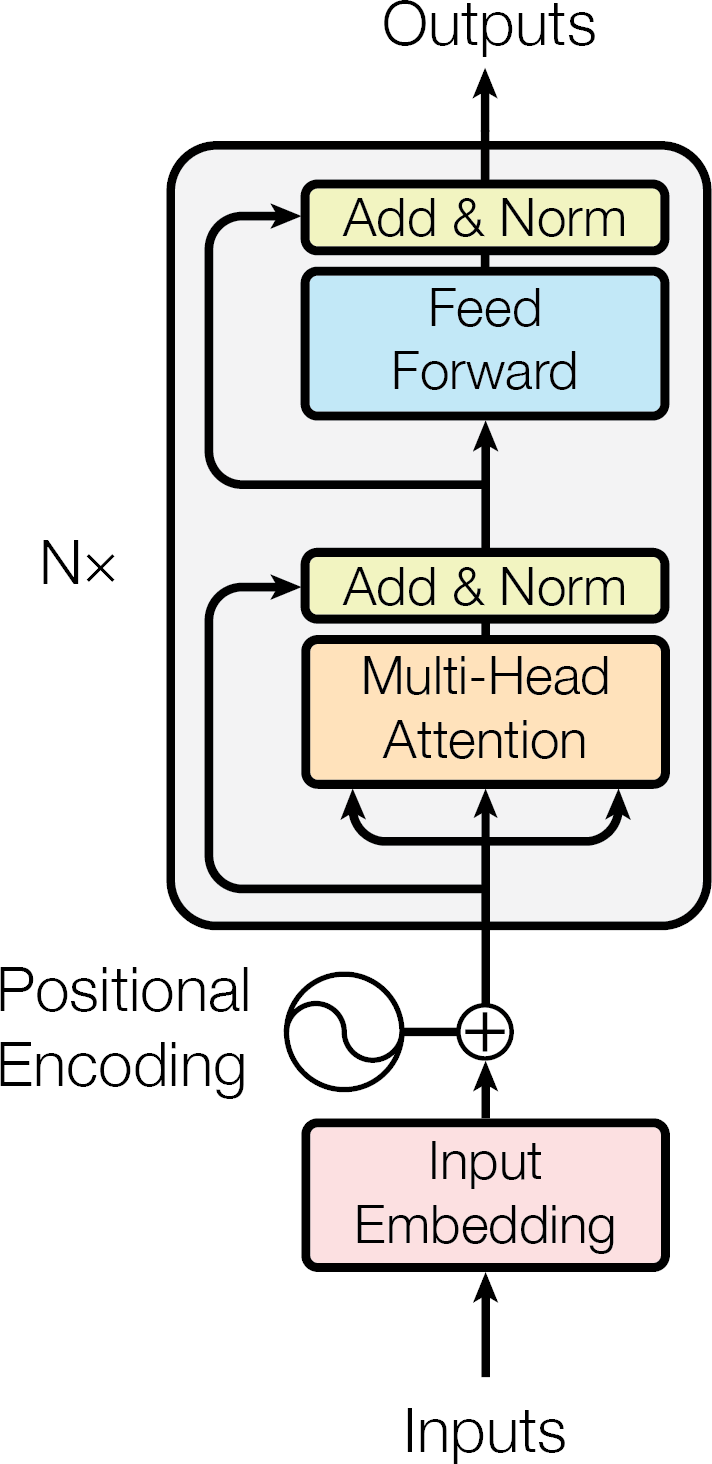
\includegraphics[width=\textwidth]{images/Transformer/TF_Encoder.png}

      \caption{Overview Transformer Encoder.}
      \label{fig:encoder}
    \end{subfigure}
    \hspace{0.1\textwidth}
    \begin{subfigure}{0.3\textwidth}
        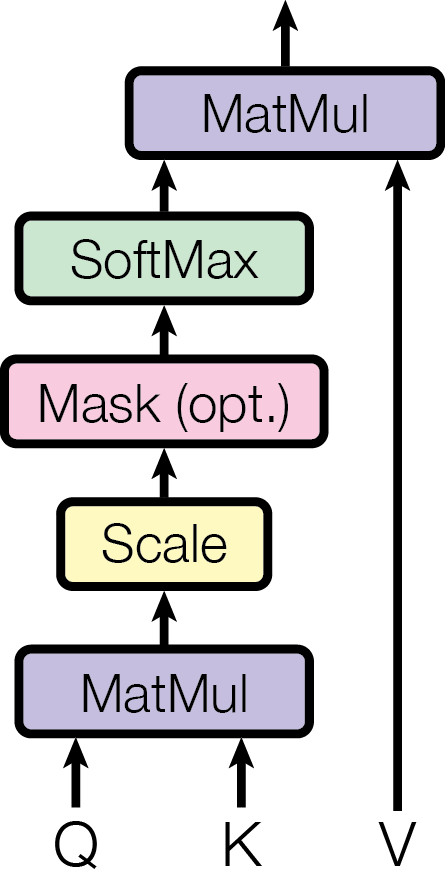
\includegraphics[width=\textwidth]{images/Transformer//AttentionHead.png}
        \caption{Attention Mechanism.}
      \label{fig:selfattention}
    \end{subfigure}
    \caption{Transformer Encoder Architecture \cite{transformer}.}
    \label{fig:main}
  \end{figure}

The idea of attention can be explained as follows: given a set of inputs, the model learns to assign a weight to each input based on its relevance to the 
task at hand.
This weighted sum of inputs is then used as a representation of the input sequence. This mechanism allows the model to focus on the most important 
parts of the input sequence while ignoring the rest.

One of the most successful architectures for attention based sequence models is the Transformer \cite{vaswani2017attention}. In the original paper, the transformer 
consists of an encoder and a decoder. For the purpose of this thesis, we are only interested in the encoder \ref{fig:encoder}, as it captures all functionality of attention based 
algorithms for sequence generation. 
The Transformer is a self-attention based model that can be used for a variety of sequence-to-sequence tasks such as machine translation,
text summarization, and language modeling.

The Transformer architecture consists of an encoder and a decoder, each containing multiple layers of self-attention and feedforward neural networks. 
The self-attention layer computes the weighted sum of all input tokens, where the weights are computed based on the similarity between the query, key and value
vectors \ref{fig:selfattention}.
The feedforward layer applies a point-wise feedforward transformation to each token separately.

In the self-attention layer, each input token is transformed into a query, key, and value vector.
These vectors are used to compute the attention weights between each pair of input tokens.
The resulting weighted sum of value vectors is used as the output of the self-attention layer.
The attention weights are computed as follows:
\begin{equation}
\text{Attention}(Q, K, V) = \text{softmax}\left(\frac{QK^T}{\sqrt{d_k}}\right)V,
\end{equation}
where $Q$, $K$, and $V$ are the query, key, and value vectors, respectively, and $d_k$ is the dimensionality of the key vectors.
The softmax function normalizes the dot product of $Q$ and $K$, which represents the similarity between the query and key vectors.
The attention weights represent the importance of each value vector in the weighted sum.\\
The vectors $Q$, $K$ and $V$ are computed using a position wise feed forward network with ReLU activation:
\begin{equation}
    QKV = \text{ReLU}(x \ W_1 + b1)W_2 + b_2
\end{equation}
, where the same weights $W_n$ and biases $b_n$ are used for every input $x$ of the sequence. This is expected to be an advantage following the BIC argument from \ref{COD}.  
However with this setup, the model has no way to encode the relative position of the tokens, which is why a positional encoding is added along the sequence dimension, 
using sin and cosin functions, to break the symmetry. \\
One advantage of the Transformer architecture is that it does not suffer from the problem of vanishing or exploding gradients.
This is because the self-attention mechanism allows the model to directly access any input token, without the need for recurrent connections.
Thus, the Transformer can process input sequences in parallel and does not suffer from the long-term dependencies problem that plagues RNNs. Self attention type 
architectures have been shown to outperform recurrent networks on a number of sequence based tasks. For example they are used in the GPT-3 architecture, which has 
shown impressive results the natural language prediction \cite{https://arxiv.org/abs/2005.14165}. While they were developed for natural language tasks, they have 
shown promising results in a multitude of areas, including image generation, image classification, imitation learning and reinforcement learning.